% !TEX root = Thesis.tex

\section{Conclusions and Limitations}


In this final section, the findings from theoretical and empirical research will be summarized and put into context. The research question from section \ref{sec:Intro} will be answered. In the following paragraphs, some common objections to offshoring will be explored, before reviewing the method used in the thesis.

\paragraph{Summary of findings}
In figure \ref{fig:ThesisResults}, the main points from literature research, empirical work and their connection are shown. On the bottom layer, the reasons for differences in offshoring that result from literature research are listed. Hereby, neighboring triangles are connected to each other. Those with a horizontal base are a prerequisite for the inverted triangles. In an analogous manner, the second layer shows the results that have been uncovered in the expert interviews. The arrangement of the triangles shows, again, relations between neighboring elements.

\begin{figure}[htb]
	\centering
	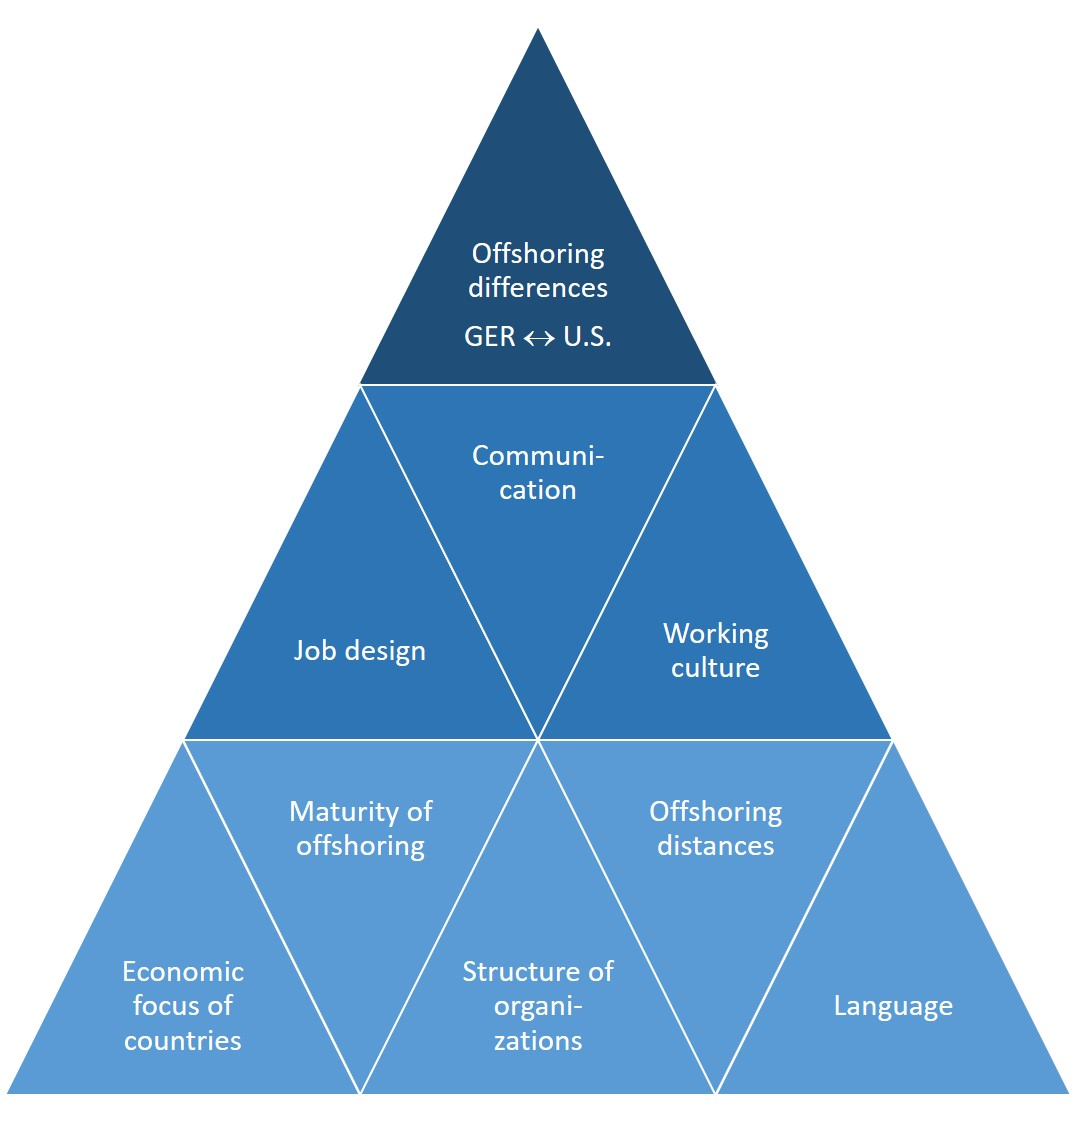
\includegraphics[width=0.8\textwidth]{Pictures/Results}
	\caption{Findings from literature research and expert interviews}
	\label{fig:ThesisResults}
\end{figure}

For example, the high maturity of offshoring in the U.S. is rooted in the prevalence of very large companies (structure of organizations) and the import focus of U.S. economy as shown in section \ref{sec:OffshoringUS}. Job design from the layer above is another important facilitator to the maturity of offshoring and a prerequisite to the unique style of communication U.S. companies use when dealing with an offshore service provider.

For Germany, the focus on exports and high influence of \gls{sme} have held back the development of offshoring, therefore the maturity is low compared to the U.S.. The holistic design of German jobs is another obstacle for offshoring, but facilitates the building of stable, long-term working relationships as detailed in the interviews with Subir Purkayastha and Ingo K\"ummritz.

The other side of the pyramid shows similar connection between its elements. English being spoken by over 1.5 billion people worldwide (see section \ref{sec:DifferencesUSGER}) facilitates offshoring over far distances. Larger corporations are better able to manage the distribution of tasks over such high distances, because of the scale such ventures tend to have. Collaborating across large distances is a big part of working culture in the U.S., which facilitates offshoring across larger distances. This, again, contributes to the communication style of U.S. companies.

For German companies, on the other hand, language is a huge roadblock to offshoring. This results in the preference for nearer offshoring locations such as East European countries, where German is more widely spoken than in farshore destinations such as India or Malaysia. Also, dealing with culturally closer service providers is easier for \gls{sme}. Working culture is another factor for nearer offshoring locations, because direct communication via phone is very natural in German offices. Large time zone differences would be hindering these exchanges. As suggested in the last sentences, German working culture has a significant impact on communication between customer and service provider.

In the introduction, a research question has been presented. The four paragraphs summarize the results of this thesis, but this is the concise answer to the research question:

\begin{quote}
	\centering
	Differences in IT offshoring between Germany and the U.S. are mostly the maturity of offshoring as well as differences in communication to the service provider. The reasons for these differences are different economic focuses, organizational structures, languages, job designs and working cultures in both countries.
\end{quote}


\paragraph{Criticism of offshoring}
This thesis has been written with the assumption that offshoring is beneficial both for companies and the participating countries. While there is a substantial body of research supporting this assumption, as shown in section \ref{sec:Theory} there are also critical voices. 

\cite{Heim.2014}, see a trend in Germany that offshoring has often been reversed since the financial crisis in 2007 and cite reasons such as customer's requirements of local production, the benefits of physical and cultural proximity of customers, product development and production, or agility of the supply chain.

On the other hand, \cite{Smite.2015}, conducted an analysis of over 500 research papers on software development offshoring. The evidence found was not reliable for deciding whether offshoring of software development tasks leads to cost savings or not. Most authors of reviewed papers did not provide actual cost savings nor the necessary data for calculating cost savings such as salaries, staff counts, or productivity. The paper concludes that companies need to plan thoroughly and include considerations other than salary level into their offshoring venture. 

The third point of criticism that is often raised by unions or the general public is the morality of offshoring. \cite{Schroder.2013}, presents two case studies of companies that had been the same company once, but got split and one half was sold to an investor, while the owning family kept the other half. So both companies were similar in power relations between unions and management as well as economic status, but management was different: the outside investor had no ties to the region where the companies are located, while the family business had very strong social ties to the region. The case studies showed that, while moral arguments did not change made decisions after the fact, they did influence what the actors defined as being in their economic interest. The social environment can influence business leaders what they perceive as economically rational.


\paragraph{Review of research method}
Of course, the scope of empirical research in this thesis is limited to the available experts. Even though the experts have covered a wide array of view points as discussed in section \ref{sec:Summary}, interviewing other or additional experts may have yielded entirely different results.

Still, the chosen method of qualitative interviews was very successful in achieving the goal of facilitating a structured knowledge transfer from the interviewee, while allowing for a natural flow of conversation and catering to the different experiences and characters of experts.

\paragraph{Consequences for German companies}
The results of the thesis, and particularly of the expert interviews, are very interesting for German companies that are interested in offshoring. They can help to understand common issues in offshoring and their root causes, and show ways to improve the offshoring potential of a company. 

Differences in offshoring between German and U.S. companies are not only a matter of different maturity, but German companies have very characteristic strengths they can take advantage of in order to successfully offshore, especially in the areas of application management and support. 






